\section{Pomysł}

\hypertarget{Toc448677644}{}

\bigskip

% KSIŻKA ZWIELOKROTNIENIE UMYSUłU
    \newline
    \akapit
    Idea projektu \ \
    \textbf{text}{JugglingMath}
    \textit{Zwielokrotnianie umysłu}
    \cite{jugglinggoodforbranin}
    footnote exapmle\footnote{http://libraryofjuggling.com/Tricks/3balltricks/Cascade.html},  \newline
    text text text text
    \glsow{wycieki pamieci}. %     
    \say{hello}
\bigskip


\bigskip

Enumerate example

\begin{enumerate}
\item Wykrywanie czy żongluje i jakim sposobem to robię,
ze względu na to, że:
    \begin{itemize}
        \item kamery montowane w laptopach czy zewnętrze do  
        \acrshort{pc}
        są coraz lepszej
        jakości, jednak przy nieodpowiednim świetle
        odwzorowywanie kolorów znacząco spada
        \item brak kamery podczerwieni, mierzącej odległość każdego
        piksela obrazu, zawęża możliwość wykrywania obrazu tylko
        do otoczenia gracza w idealnym
        świetle i kontrastowych kolorach piłeczek
    \end{itemize}
\item Wykrywanie czy udzieliłem dobrej odpowiedzi, gdyż:
    \begin{itemize}
        \item w większości przypadków urządzenia do rejestrowania
        dzwięku w komputerach są niskiej jakości
        \item zdarzają się \say{duże} opóźnienia w przesyłaniu
        dźwięku przez przeglądarkę
    \end{itemize}
\end{enumerate}

\newpage

% SCREENSHOOT APLIKACJA WEBOWA JUGGLING MATH
\begin{figure}[h]
    \caption{Aplikacja webowa \textit{JugglingMath}.}
    \centering
    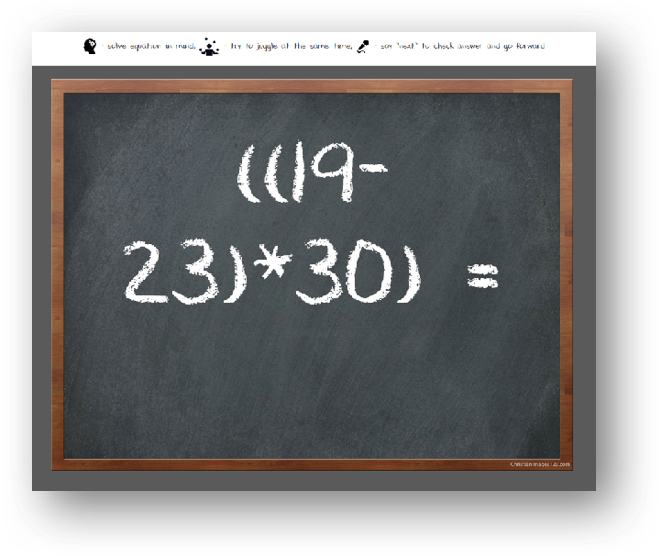
\includegraphics[width=5.1614in]{graphics/webapp_jm.png}
    \label{webappJugglingMathScreenshot}
\end{figure}

\subsection{Kinect}

% DLACZEGO KINECT IDEALNY

    \newline
    \akapit
    Rozwiązaniem moich problemów okazał się sensor ruchu Microsoft
    Kinect{\textregistered}~\ref{sensorFrontPic},
    wprowadzony na rynek w 2010 roku
    dla konsoli Microsoft Xbox{\textregistered} i
    umożliwiający jej użytkownikom
    sterowanie interfejsem w naturalny sposób, za pomocą ruchów i gestów.
    %
    Kompatybilność sensora ze zwykłym \acrshort{pc} z Microsoft
    Windows{\textregistered} zaopatrzonego w Kinect \acrshort{sdk} umożliwiał mi
    napisanie aplikacji nie posiadając konsoli XBox i zrobienie
    dokładnie tego co chciałem, czyil rejestrowaniae obrazu
    wraz z odległością każdego pixela~\ref{kinectDeviceSchema}.
    %
    Ponadto sprzętowo zaprogramowane rozpoznawania
    szkieletu  gracza~\ref{kinectSkeletonJointsPic}
    oraz bogate \acrshort{api} dało mi szerokie pole do manewru oraz pewność,
    że napisany kod będzię mógł posłużyć w przyszłości do stworzenia
    aplikacji uruchamianej wprost z konsoli Xbox.


% Picture example
\begin{figure}[h]
    \centering
    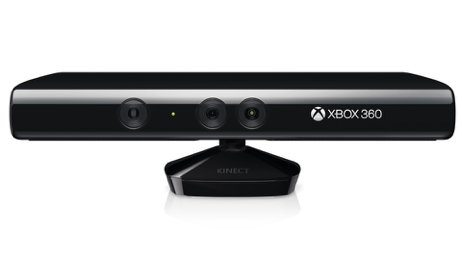
\includegraphics[width=1.7614in,height=1.0579in]{graphics/kinect.png}
    \caption{Sensor Kinect dla XBox360.}
    \label{sensorFrontPic}
\end{figure}

\bigskip

Table example

\begin{table}[h!]
    \centering
    \begin{tabular}{||c c||}
        \hline
        Element & Wielkość zajmowanej pamięci w megabajtach \\ [0.5ex]
        \hline\hline
        %
        Depth Short Array
        \footnote{Tablica głębokości pikseli, o długości 307 200 przy
        rozdzielczości 640x480 i typie short (2 bajty na piksel).}
        & 0.6144 \\
        %
        Color Bytes Array
        \footnote{Tablica kolorowego obrazu, o długości 1 228 800
        przy 640x480 i typie byte (4 bajty na piksel).}
        & 1.2288 \\
        %
        20 frames of color
        & 12.288 \\
        %
        %
        30 frames of color
        & 18.432 \\
        %
        20 seconds of recorded color stream
        & 368.46 \\
        \hline
    \end{tabular}
    \caption{Teoretyczne zużycie pamięci.}
    \label{memoryConsumption}
\end{table}
